\documentclass[11pt,a4paper]{article}
\usepackage[T1]{fontenc}
\usepackage[margin=1in]{geometry}
\usepackage{amsmath,amssymb,mathtools}
\usepackage{booktabs}
\usepackage{graphicx}
\usepackage{xcolor}
\usepackage[colorlinks=true,linkcolor=blue!60!black,citecolor=blue!60!black,urlcolor=blue!60!black]{hyperref}
\usepackage{microtype}
\usepackage{xurl}
\setlength{\emergencystretch}{3em}
\usepackage{enumitem}
\usepackage[most]{tcolorbox}
\newtcolorbox{keybox}[1][]{colback=blue!3,colframe=blue!45!black,boxrule=0.5pt,left=4pt,right=4pt,top=3pt,bottom=3pt,#1}
\newtcolorbox{failbox}[1][]{colback=red!3,colframe=red!45!black,boxrule=0.5pt,left=4pt,right=4pt,top=3pt,bottom=3pt,#1}
\hypersetup{pdftitle={Gated exciton fluids IV},pdfauthor={Xavier Callens},pdfsubject={Dimensional lifting, sliding walls and relaxed point sets: negative results}}

\begin{document}
\begin{center}
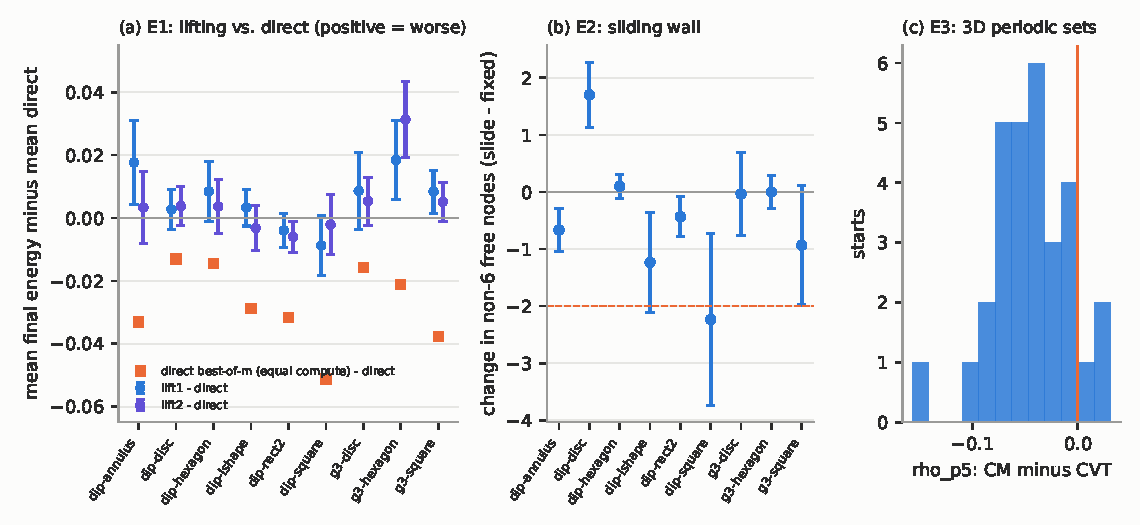
\includegraphics[width=0.98\textwidth]{figs_companion4/fig_dimlift.pdf}\\[2pt]
{\footnotesize (a) Mean final energy of the lifted runs minus the direct mean (valid runs, $\pm1$ s.e. of the difference); orange: best of $m$
direct restarts ($m$ = evaluation ratio of lift1) minus the direct mean. (b) Change of the number of non-6-coordinated free nodes with
sliding walls, $\pm1$ s.e.; dashed: registered threshold $-2$. (c) Paired difference of the 5th-percentile tetrahedron radius ratio,
CM minus CVT, 30 starts.}
\end{center}
\vspace{-0.6em}
\begin{center}
{\Large\textbf{Gated exciton fluids IV:}\\[2pt]
\large three heuristics tested and not confirmed: dimensional lifting, sliding walls,\\ and completely monotone relaxation as a 3D mesh generator}\\[8pt]
Xavier Callens\\ {\small SocrateAI Research \quad\url{https://github.com/xaviercallens/SocrateAI-Scientific-QuantumFluids}}\\[2pt]
{\small October 2026}
\end{center}
\vspace{-0.4em}

\begin{abstract}\small\noindent
After papers~I--III~\cite{CallensI,CallensII,CallensIII}, three ideas that had been suggested for the classical node-arrangement
problem were pre-registered and tested with a plain numpy L-BFGS engine on the container geometries of the Fenris study:
\textbf{(E1)} lifting the particles to $2+k$ dimensions and annealing the extra coordinates away, as an optimisation aid;
\textbf{(E2)} letting the wall nodes slide along the wall; \textbf{(E3)} using a completely monotone repulsion in a periodic cube as a
3D mesh generator, against Lloyd/centroidal Voronoi relaxation. Results: E1 shows no benefit at equal compute in any of the nine
shape--kernel cases (30 starts each); E2 reduces the number of non-sixfold-coordinated nodes by 2 or more in one of nine cases and
increases it significantly in one; E3 is slightly \emph{worse} than CVT in the 5th-percentile tetrahedron radius ratio (30 paired starts).
All three registered gates are not met. The runs are small ($N_{\rm free}\approx60$ in 2D, $N=216$ in 3D), single-engine and
classical, and say nothing about excitons, string theory or the universal-optimality theorem. Written with an AI system; not refereed.
\end{abstract}

\section{What was tested, and why}

The suggestions came from a brainstorm that borrowed vocabulary from string theory: ``lift to 8D or 24D where the optimum is
perfect and project back''; Kaluza--Klein ``dimensional hopping''; boundaries as flexible branes. Our own analysis (the project
note in the repository) concluded that no theorem transports the optimality of $E_8$ or the Leech lattice to 3D and that the
difficulty of N-body minimisation is the number of local minima, not the dimension. What survives as a testable statement is
modest: whether extra coordinates help a local optimiser escape defective minima, whether giving the wall extra freedom reduces
frustration at the boundary, and how a relaxed CM point set compares as a mesh with the standard CVT. All three were registered
before the first run (\texttt{exploration/exciton/dimlift/PREREG.md}); three amendments (A1: container penalty and failure rule,
A2: $N=216$ for E3, A3: a speed-only vectorisation) are dated.

\begin{keybox}
\textbf{Scope.} Containers, wall nodes (spacing $0.5$), random-sequential-addition starts and the defect analysis are those of the
Fenris study, imported unchanged; the optimiser is a new numpy L-BFGS code. Kernels: the ungated dipole $2/r-2/\sqrt{r^2+d^2}$
($d=0.5$) and the gated kernel $D/d=3$ (Poisson series, tabulated). Shapes: square, hexagon, disc, $2{:}1$ rectangle, L-shape, annulus
(gated kernel on square, hexagon, disc only); $N_{\rm free}\approx60$; 30 starts each, shared across methods. No claim is made
about excitons.
\end{keybox}

\section{E1: dimensional annealing}

\textbf{Method.} The same starts are relaxed directly in 2D, or lifted to $2+k$ dimensions ($k=1,2$; extra coordinates
$\mathcal N(0,0.1^2)$; pair energy a function of the lifted distance; wall nodes at $w=0$), with a quadratic confinement
$\lambda|w|^2$ stepped through six values and 150 L-BFGS iterations per stage, then a 2D polish. \emph{A point wall leaks into the
extra dimensions}: in development runs 15 of 60 nodes left the container, so the lifted problem uses a container$\times\mathbb R^k$
penalty and a projection after each stage (amendment A1). A run with any node outside the container at the end is a failed run
(counted, energy excluded; the rule is the same for every method and only the lifted ones fail): 7 of 30 (square, $k=1$) and 8 of 30 (square, $k=2$) fail, and 1--4 on the $2{:}1$ rectangle and the L-shape; none elsewhere.
The equal-compute control is the best of $m$ direct restarts with $m$ the evaluation ratio (6--17).

\textbf{Result.} Lifting costs 6--17 times more evaluations per start (12--30 times in wall-clock). In none of the nine cases is the mean
final energy lower than direct by two standard errors, and in no case does lifting beat the equal-compute control (the best-of-$m$
direct mean is lower than the lifted mean in all nine; panel a). The control is not tilted against lifting: every asymmetry favours
it (failed lifted runs consume compute but are not penalised; the best-of-$m$ bootstrap is capped at the sample minimum; the lifted
failures come from the final polish of the harness and concentrate on shapes with corners). The fraction of starts reaching the best
energy found among the fixed-wall methods (direct/lift1/lift2) is: annulus $0.43/0.40/0.53$, disc $0.50/0.40/0.33$, hexagon
$0.03/0.07/0.10$, L-shape $0.00/0.07/0.10$, $2{:}1$ $0.03/0.00/0.03$, square $0.23/0.27/0.17$; gated: disc $0.43/0.37/0.27$, hexagon
$0.07/0.03/0.00$, square $0.27/0.17/0.13$. With 30 starts these differences are within sampling noise and have no consistent sign (the
registered ``fraction not lower'' conjunct holds in three of nine cases for lift1 and in four of nine for lift2); for gated hexagon, lift2 is
significantly worse than direct in a paired comparison ($t\approx-3$). The number of distinct minima (1e-6 relative) is similar across methods
(e.g.\ square 13/12/13, L-shape 20/23/15). The registered gate (dipole kernel: lower mean by more than $2$ s.e.\ on at least four of six
shapes, fraction not lower, and surviving the control) is \textbf{not met}.

\section{E2: sliding walls}

\textbf{Method.} Non-corner wall nodes slide along their ring (arclength parameter) with the wall--wall repulsion included, same starts;
energies are total energies including the wall--wall term. The sliding problem is a superset of the fixed-wall one, so its minimum
energy is lower \emph{by construction}; the informative quantity is the change of the defect count.

\textbf{Result.} The mean change in the number of non-6-coordinated free nodes (slide minus fixed; $\pm$ one standard error) is: square $-2.2\pm1.5$,
L-shape $-1.2\pm0.9$, annulus $-0.7\pm0.4$, $2{:}1$ rectangle $-0.4\pm0.4$, hexagon $+0.1\pm0.2$, disc $+1.7\pm0.6$ (dipole kernel);
gated: square $-0.9\pm1.0$, hexagon $0.0\pm0.3$, disc $0.0\pm0.7$. The registered gate (decrease of at least two on at least
three of six shapes) is \textbf{not met}: it is met on one (square, $-2.2\pm1.5$: the mean is $0.15$ s.e.\ from the threshold and $1.5$ s.e.\ from zero, so
not itself significant), and the disc gets \emph{worse} by about three standard errors. The mean total energy change (slide minus fixed) is
negative in seven of nine cases (largest: L-shape $-0.087$, gated square $-0.079$) but \emph{positive} on the disc ($+0.010$) and the
annulus ($+0.0025$): the sliding problem contains the fixed one, so these are local minima, not global ones. The net topological
charge $Q$ changes in 0--40\% of starts depending on the shape, against the registered expectation that it would not; we did not test
why (the Gauss--Bonnet identity fixes $Q$ given the boundary coordination, which sliding changes, but this is an interpretation).

\section{E3: a CM-relaxed periodic point set as a 3D mesh}

\textbf{Method.} $N=216$ points in the periodic unit cube (30 starts) are relaxed (a) with the screened repulsion $e^{-kr}/r$,
$kL=6$ (minimum image, shifted cutoff at $L/2$), or (b) by 40 Lloyd/CVT iterations with $1.5\times10^5$ Monte-Carlo samples; Poisson
points are the reference. Delaunay tetrahedra of the $3\times3\times3$ tiling restricted to the central cell are scored by the
radius ratio $3r_{\rm in}/R$ and the minimum dihedral angle.

\textbf{Result.} Both relaxations are far better than Poisson (median 5th-percentile radius ratio 0.20 for Poisson, 0.63 for CM, 0.68
for CVT; fraction of tetrahedra with radius ratio $<0.3$: 12\% for Poisson, 0.5\% for both relaxations). CM is below CVT in the
5th-percentile radius ratio by $0.045\pm0.007$ (paired mean $\pm$ s.e., from the per-seed records) and beats it in 3 of 30 paired starts;
the gate (24 of 30) is \textbf{not met}. The picture is not one-sided: CM is \emph{better} on the worst-case metrics (median minimum radius ratio
0.112 against 0.086; median minimum dihedral angle $5.9^\circ$ against $4.4^\circ$) while CVT is better on the 5th-percentile
radius ratio and dihedral angle ($36.8^\circ$ against $35.0^\circ$); the registered gate concerned only the former. The kernel
parameter $kL=6$ was fixed in advance and not tuned; a different screening length may change the margin, which was not tested.

\section{What this does and does not show}

\begin{itemize}[leftmargin=1.2em,itemsep=1pt]
\item The lifted problem is more expensive and no better at equal compute for these small, strongly confined instances. This does
not exclude a benefit for other problem classes (the rank-relaxation literature is about different landscapes) or much larger $N$.
\item Sliding walls help one shape marginally and hurt another significantly; no general statement is supported. No buckling into a
third dimension was tested.
\item CM relaxation is a good point-set regulariser but not better than CVT as measured; nothing is shown about conforming
meshes of CAD domains, size grading or boundary recovery.
\item None of this involves the lattice-optimality theorem, whose planar statement remains unrefereed and AI-generated.
\end{itemize}

\textbf{Process and deviations.} The development runs (square seeds 0--5, E3 seed 0) are inside the registered sets and
amendment A1 tuned the lifted-run parameters on them. The CVT used $1.5\times10^5$ Monte-Carlo samples per iteration, not the registered
$2\times10^5$ (not amended; disclosed in the erratum of the pre-registration). Records are in \texttt{exploration/exciton/dimlift/results/}; a first set of 76 disc runs produced with a slow
nearest-edge search was discarded and the disc rerun from scratch after the speed-only amendment A3. The change is numerically equivalent, not identical: on the square it is bit-identical
(18 runs rechecked), on the disc `direct' and `slide' are bit-identical but 15 of 37 lifted runs end in a different local minimum (up to
0.12 in energy), so the discarded 76 runs are a usable replicate. The square and hexagon runs predate A3 and are kept. The numbers in this paper are generated by \texttt{analyse.py} (\texttt{summary.json}); the
verifier notes of papers II--III and the independent review of this paper are in \texttt{docs/designs/EXCITON\_FLUID\_VERIFIER\_NOTES\_*.md}.

\begin{thebibliography}{9}\small
\bibitem{CallensI} X. Callens, \emph{Gated exciton fluids}, Zenodo, \url{https://doi.org/10.5281/zenodo.23294615} (2026).
\bibitem{CallensII} X. Callens, \emph{Gated exciton fluids II}, Zenodo, \url{https://doi.org/10.5281/zenodo.23297479} (2026).
\bibitem{CallensIII} X. Callens, \emph{Gated exciton fluids III}, Zenodo, \url{https://doi.org/10.5281/zenodo.23298292} (2026).
\end{thebibliography}
\end{document}
